% ============================================================
%  Computer Graphics Laboratory Report Template
%  Requirements: TNR 12pt, 1.5 spacing, specific margins
% ============================================================
\documentclass[12pt, a4paper]{report}
\usepackage{lab_report}

% ============================================================
%  DOCUMENT METADATA — edit these fields
% ============================================================
\newcommand{\ReportTitle}{Laboratory Work No. 3}
\newcommand{\ReportSubtitle}{Empirical analysis of algorithms: Depth First Search (DFS), Breadth First Search(BFS)}
\newcommand{\StudentName}{Cristian Bruma}
\newcommand{\GroupName}{FAF-242}
\newcommand{\SupervisorName}{asist. univ.  Cristofor Fiștic}
\newcommand{\Ministry}{Ministerul Educaţiei și Cercetării al Republicii Moldova}
\newcommand{\UniversityName}{Universitatea Tehnică a Moldovei}
\newcommand{\DepartmentName}{Facultatea Calculatoare, Informatică și Microelectronică}
\newcommand{\AcademicYear}{2026}

% ============================================================
\begin{document}

% ── TITLE PAGE ───────────────────────────────────────────────
\begin{titlepage}
  \thispagestyle{empty}        % no page number displayed on title page
  \begin{center}
    \textbf{\MakeUppercase{\Ministry}}\\[4pt]
    \textbf{\MakeUppercase{\UniversityName}}\\[4pt]
    \textbf{\MakeUppercase{\DepartmentName}}\\[40pt]

    \rule{\linewidth}{0.5pt}\\[6pt]
    {\Large\bfseries\MakeUppercase{\ReportTitle}}\\[4pt]
    {\large\bfseries\ReportSubtitle}\\[6pt]
    \rule{\linewidth}{0.5pt}\\[30pt]

    {\Large Laboratory Report}\\[4pt]
    {\Large Analysis of algorithms}\\[60pt]
  \end{center}

  \begin{flushleft}
    \begin{tabular}{ll}
      \Large\textbf{Student:}    & \Large\StudentName \\
      \Large\textbf{Group:}      & \Large\GroupName   \\
      \Large\textbf{Supervisor:} & \Large\SupervisorName \\
    \end{tabular}
  \end{flushleft}

  \vfill
  \begin{center}
    \Large\textbf{Chișinău, \AcademicYear}
  \end{center}
\end{titlepage}

% Title page IS counted in pagination (page 1) but number not shown.
\setcounter{page}{1}

% ── TABLE OF CONTENTS ────────────────────────────────────────
\newpage
\renewcommand{\contentsname}{TABLE OF CONTENTS}
\renewcommand{\cfttoctitlefont}{\hfill\fontsize{13pt}{15pt}\bfseries}
\renewcommand{\cftaftertoctitle}{\hfill}
\tableofcontents
\thispagestyle{plain}          % show page number on ToC page

% ============================================================
%  CHAPTER 1 — INTRODUCTION
% ============================================================
\chapter{ALGORITHM ANALYSIS}

\section{Objective}

Empirical analysis of algorithms: Depth First Search (DFS), Breadth First Search(BFS).

\section{Tasks}


\begin{dashenum}
  \item Implement the algorithms listed above in a programming language;
  \item Establish the properties of the input data against which the analysis is performed;
  \item Choose metrics for comparing algorithms;
  \item Perform empirical analysis of the proposed algorithms;
  \item Make a graphical presentation of the data obtained;
  \item Make a conclusion on the work done.
\end{dashenum}

\section{Theoretical Notes}

Breadth First Search (BFS) and Depth First Search (DFS) are two fundamental
graph traversal algorithms used to systematically visit all vertices of a graph.
BFS explores the graph level by level, starting from a source vertex and visiting
all its immediate neighbours before proceeding to vertices at the next depth
level~\cite{ref:bfs}. This behaviour is achieved using a queue data structure,
which ensures that vertices are processed in the order they are discovered.
As a result, BFS guarantees the shortest path (in terms of number of edges)
between the source and any reachable vertex in an unweighted graph.

DFS, in contrast, explores as far as possible along each branch before
backtracking~\cite{ref:dfs}. It is implemented either recursively or
iteratively using a stack. DFS is particularly suited for tasks such as
cycle detection, topological sorting, and finding connected components.
The time complexity of both algorithms is $O(V + E)$, where $V$ represents
the number of vertices and $E$ the number of edges in the graph~\cite{ref:yt}.
The space complexity depends on the structure of the graph: BFS requires
$O(V)$ space for the queue, while DFS requires $O(V)$ space for the
recursion stack in the worst case.

\section{Introduction}

Graph traversal is the process of visiting every vertex in a graph in a
systematic and well-defined order. The two most foundational algorithms
for this purpose are Breadth First Search (BFS) and Depth First Search
(DFS), both of which form the basis of countless more advanced algorithms
in computer science. A graph $G$ is formally defined as a pair $G = (V, E)$,
where $V$ is a set of vertices and $E$ is a set of edges connecting pairs
of vertices. The problem of traversing such a structure efficiently has
been studied since the earliest days of discrete mathematics and computer
science.

DFS traces its theoretical roots to the work of French mathematician
Charles Pierre Trémaux in the 19th century, who devised a strategy for
solving mazes by exploring each path as deeply as possible before
backtracking — a principle identical to that of modern DFS. The formal
algorithmic treatment of depth-first traversal was later established by
John Hopcroft and Robert Tarjan in the 1970s, whose work on DFS-based
algorithms earned them the Turing Award in 1986. BFS, on the other hand,
was formally described by Konrad Zuse in his 1945 thesis, and later
reinvestigated by Edward F. Moore in 1959 in the context of finding the
shortest path out of a maze. It was further formalized by C. Y. Lee in
1961 for wire routing in circuit boards.

Both algorithms operate on the same input — a graph and a starting vertex
— yet differ fundamentally in the order in which vertices are explored.
BFS expands outward layer by layer using a queue, guaranteeing the
shortest path in unweighted graphs, while DFS plunges deep into the
graph using a stack or recursion, making it better suited for structural
analysis tasks such as cycle detection, topological sorting, and strongly
connected component identification. The time complexity of both algorithms
is $O(V + E)$, making them equally efficient in terms of asymptotic growth.

With the evolution of computer science and algorithmics, both traversal
strategies have been applied and optimized across a wide range of domains,
from web crawling and social network analysis to compiler design and
artificial intelligence. As mentioned previously, the performance of an
algorithm can be analyzed mathematically, through formal derivation, or
empirically, through experimental observation and measurement. Within
this laboratory, the empirical performance of BFS and DFS will be
analyzed by measuring execution time across graphs of varying sizes and
structures, with the aim of observing how theoretical complexity
manifests in practice.

\section{Comparison Metric}

The comparison metric for this laboratory work will be considered the time of execution of each 
algorithm $(T(n))$

\section{Input Format}

The algorithms will be applied on 2 sets, each containing 10 graphs with vertex numbers uniformly distributed within the interval [100:16000].
The first set will contain randomly generated graphs of sparse category, in this particular laboratory work, a sparse graph is implemented as a graph with average degree 8.
The second set will contain randomly generated graphs of dense category, in this particular laboratory work, a dense graph is implemented as a graph containing 25\% edges out of maximum possible amount.

% ============================================================
%  CHAPTER 2 — MATERIALS AND METHODS
% ============================================================
\chapter{IMPLEMENTATION}

\section{DFS}

The Depth First Search (DFS) algorithm was implemented for three different graph representations: adjacency matrix, adjacency list, and edge list. The implementation supports disconnected graphs by iterating through all vertices and starting a new traversal from each unvisited vertex.

The recursive DFS function for adjacency matrix is defined as follows:

\begin{lstlisting}[language=C++, caption={DFS for adjacency matrix (recursive helper)}]
void dfs_adj_matrix(const std::vector<std::vector<bool>>& matrix, 
                    std::vector<bool>& visited, int node){
    visited[node] = true;
    int n = visited.size();
    for(int i = 0; i < n; i++) {
        if(matrix[node][i] && !visited[i]) 
            dfs_adj_matrix(matrix, visited, i);
    }
}
\end{lstlisting}

The wrapper function that handles disconnected components is:

\begin{lstlisting}[language=C++, caption={DFS for adjacency matrix (main function)}]
void dfs_adj_matrix(const std::vector<std::vector<bool>>& matrix){
    int v = matrix[0].size();
    std::vector<bool> visited(v, false);

    for (int i = 0; i < v; i++) {
        if (!visited[i]) {
            dfs_adj_matrix(matrix, visited, i);
        }
    }
}
\end{lstlisting}

\newpage

For adjacency list representation, the implementation is more efficient and cleaner:

\begin{lstlisting}[language=C++, caption={DFS for adjacency list}]
void dfs_adj_list(const std::vector<std::vector<int>>& graph, 
                  std::vector<bool>& visited, int node) {
    visited[node] = true;

    for (int neighbor : graph[node]) {
        if (!visited[neighbor]) {
            dfs_adj_list(graph, visited, neighbor);
        }
    }
}

void dfs_adj_list(const std::vector<std::vector<int>>& graph) {
    int v = graph.size();
    std::vector<bool> visited(v, false);

    for (int i = 0; i < v; i++) {
        if (!visited[i]) {
            dfs_adj_list(graph, visited, i);
        }
    }
}
\end{lstlisting}

\newpage

The edge list version scans all edges at each step to find neighbors (less efficient, $O(VE)$ in worst case):

\begin{lstlisting}[language=C++, caption={DFS for edge list}]
void dfs_edge_list(int n, const std::vector<std::pair<int, int>>& edges, 
                   std::vector<bool>& visited, int node) {
    visited[node] = true;

    for (const auto& edge : edges) {
        int u = edge.first;
        int v = edge.second;
        if (u == node && !visited[v])
            dfs_edge_list(n, edges, visited, v);
        else if (v == node && !visited[u])
            dfs_edge_list(n, edges, visited, u);
    }
}

void dfs_edge_list(int n, const std::vector<std::pair<int, int>>& edges) {
    std::vector<bool> visited(n, false);

    for (int i = 0; i < n; i++)
        if (!visited[i])
            dfs_edge_list(n, edges, visited, i);
}
\end{lstlisting}

DFS uses recursion (implicit stack) and explores as far as possible along each branch before backtracking.

\begin{figure}[ht]
  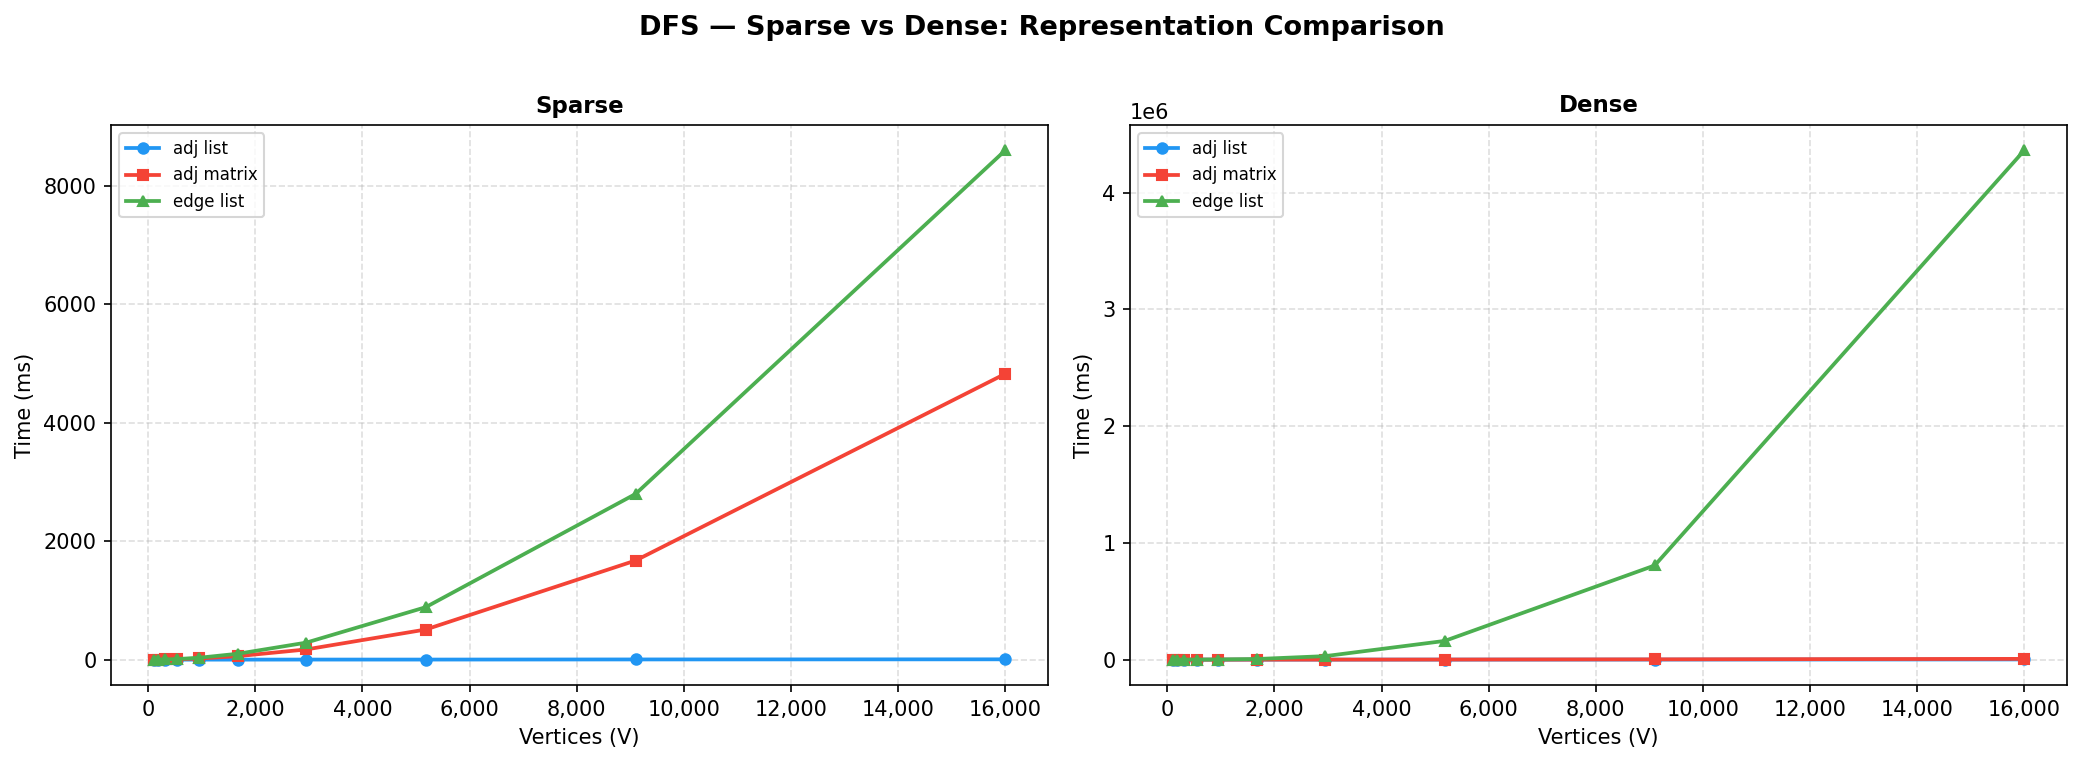
\includegraphics[width=1.05\linewidth]{dfs_representations.png}
  \caption{The result of the DFS benchmarking}
  \label{fig:dfs_representations}
\end{figure}

As seen in figure~\ref{fig:dfs_representations}, the adjacency list implementation consistently outperforms the adjacency matrix and edge list versions, especially as graph size increases, due to its more efficient representation of sparse graphs.
The experimental results confirm that the Depth-First Search (DFS) algorithm performs significantly better on sparse graphs compared to dense graphs when implemented using adjacency list representation.
On sparse graphs (average degree 8), DFS on adjacency list demonstrates excellent performance. 
For example, with 1,680 vertices, the execution time was only 5,899,900 ns, while on a dense graph of the same size it required 17,002,000 ns. 
At 16,000 vertices, DFS completed the sparse graph in 5,001,000 ns, whereas the dense graph took 1,552,035,000 ns. 
This represents a speedup of approximately 310 times in favor of the sparse graph at the largest tested size.
The difference becomes even more pronounced as the number of vertices increases. While execution time on sparse graphs grows roughly linearly, the time on dense graphs grows much faster due to the significantly higher number of edges. 
At 9,100 vertices, DFS on the sparse graph finished in 3,002,000 ns, compared to 515,000,000 ns on the dense graph — a difference of over 171 times. 
Overall, across the tested range, DFS was between 3 to 310 times faster on sparse graphs than on dense graphs of comparable vertex count, clearly demonstrating that adjacency-list-based DFS is highly efficient for graphs with low edge density.
These results align with the theoretical time complexity of $  O(V + E)  $, where the number of edges $  E  $ has a dominant impact on performance. 
Since sparse graphs contain far fewer edges, the algorithm processes significantly fewer neighbor relationships, resulting in substantially lower execution times.

\newpage

\section{BFS}

The Breadth First Search (BFS) algorithm was implemented using a queue for level-order traversal. Like DFS, it handles disconnected graphs by iterating over all vertices.

The implementation for adjacency matrix is as follows:

\begin{lstlisting}[language=C++, caption={BFS for adjacency matrix}]
void bfs_adj_matrix(const std::vector<std::vector<bool>>& matrix){
    int n = matrix.size();
    std::vector<bool> visited(n, false);

    std::queue<int> qu;
    for (int src = 0; src < n; src++) {
        if (visited[src]) continue;
        visited[src] = true;
        qu.push(src);

        while(!qu.empty()){
            int node = qu.front();
            qu.pop();
            for(int i = 0; i < n; i++){
                if(matrix[node][i] && !visited[i]){
                    visited[i] = true;
                    qu.push(i);
                } 
            }
        }
    }
}
\end{lstlisting}

\newpage

For adjacency list (most efficient among the three):

\begin{lstlisting}[language=C++, caption={BFS for adjacency list}]
void bfs_adj_list(const std::vector<std::vector<int>>& graph) {
    int n = graph.size();
    std::vector<bool> visited(n, false);
    std::queue<int> q;

    for (int src = 0; src < n; src++) {
        if (visited[src]) continue;
        visited[src] = true;
        q.push(src);

        while (!q.empty()) {
            int node = q.front(); q.pop();

            for (int neighbor : graph[node]) {
                if (!visited[neighbor]) {
                    visited[neighbor] = true;
                    q.push(neighbor);
                }
            }
        }
    }
}
\end{lstlisting}

\newpage

The edge list version is functionally correct but has $O(VE)$ time complexity due to scanning the entire edge list for every dequeued vertex:

\begin{lstlisting}[language=C++, caption={BFS for edge list}]
void bfs_edge_list(int n, const std::vector<std::pair<int, int>>& edges) {
    std::vector<bool> visited(n, false);
    std::queue<int> q;

    for (int src = 0; src < n; src++) {
        if (visited[src]) continue;
        visited[src] = true;
        q.push(src);

        while (!q.empty()) {
            int node = q.front(); q.pop();

            for (const auto& edge : edges) {
                int u = edge.first;
                int v = edge.second;
                if (u == node && !visited[v]) {
                    visited[v] = true;
                    q.push(v);
                } else if (v == node && !visited[u]) {
                    visited[u] = true;
                    q.push(u);
                }
            }
        }
    }
}
\end{lstlisting}

BFS explores the graph level by level, guaranteeing the shortest path (in number of edges) from the source to any reachable vertex in an unweighted graph.

\newpage

\begin{figure}[ht]
  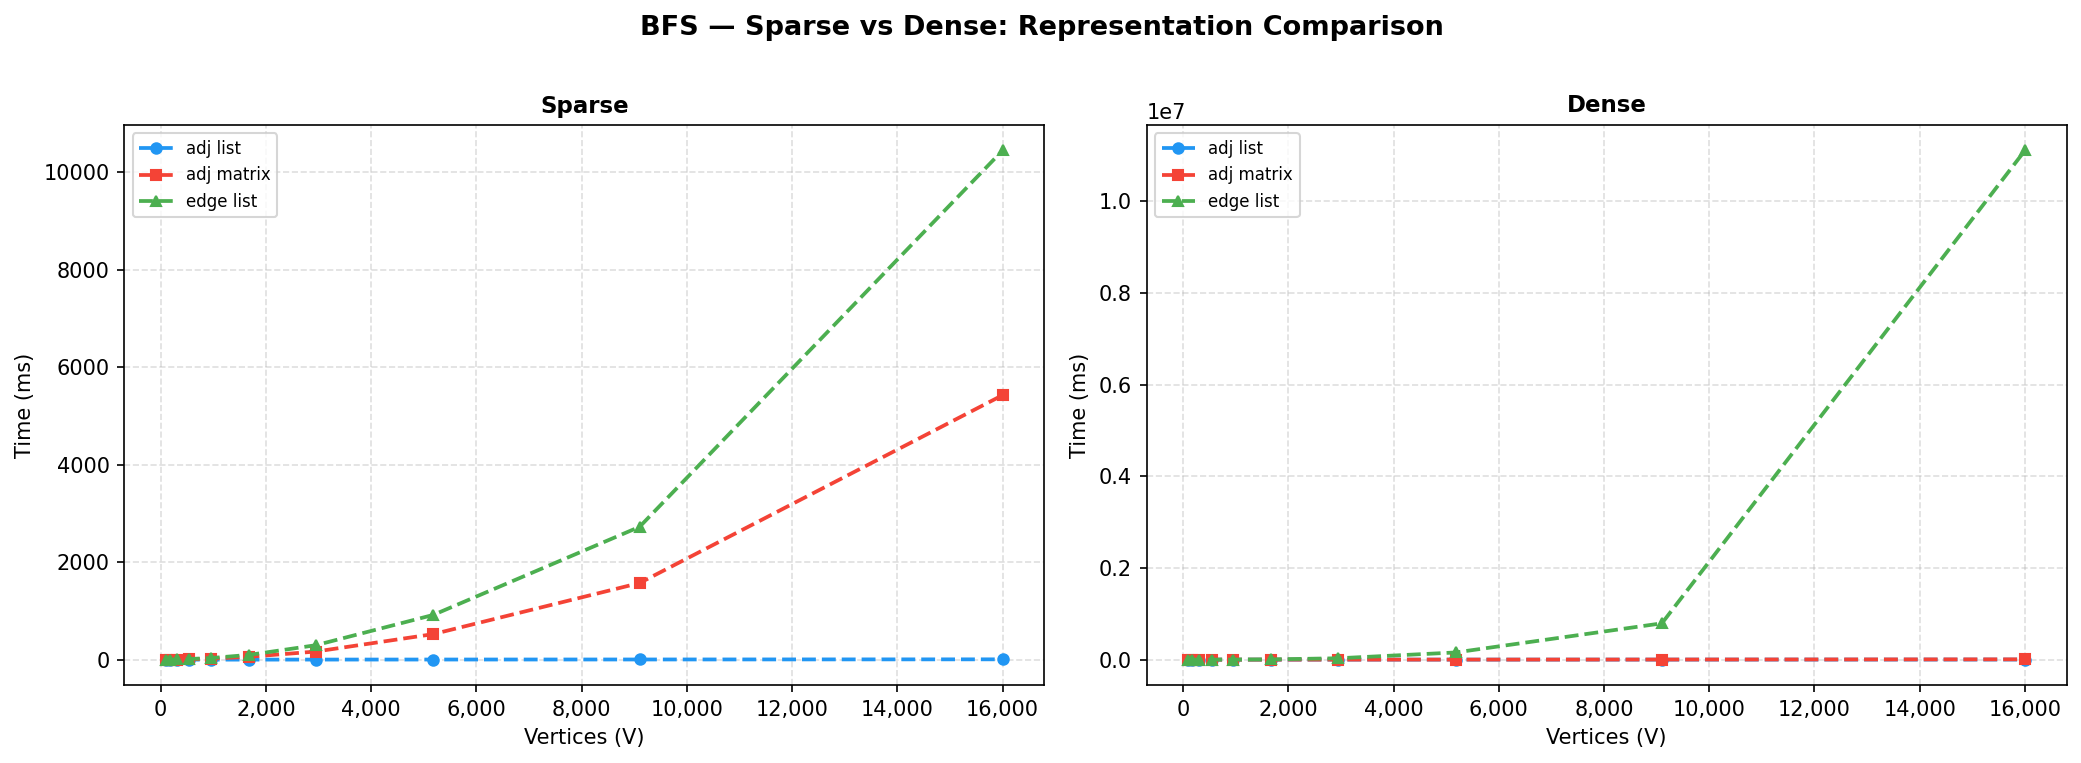
\includegraphics[width=1.05\linewidth]{bfs_representations.png}
  \caption{The result of the BFS benchmarking}
  \label{fig:bfs_representations}
\end{figure}

The experimental results show that the Breadth-First Search (BFS) algorithm, like DFS, executes considerably faster on sparse graphs compared to dense graphs when using the adjacency list representation.
On sparse graphs with an average degree of 8, BFS maintains excellent performance even for large inputs. 
For instance, at 1,680 vertices, BFS on adjacency list completed in 18,000,000 ns, while the same algorithm on a dense graph of identical size required 180,000,000 ns. 
At the largest tested size of 16,000 vertices, BFS finished the sparse graph in only 5,999,000 ns, whereas it took 1,502,997,000 ns on the dense graph. 
This corresponds to a speedup of approximately 250 times in favor of the sparse graph.
The performance gap widens rapidly with increasing graph size. 
At 9,100 vertices, BFS on the sparse graph ran in 3,000,000 ns, compared to 485,999,000 ns on the dense graph — a difference of over 162 times. 
In general, across the tested datasets, BFS was between 5 to 250 times faster on sparse graphs than on dense graphs of the same number of vertices.
This substantial difference is explained by the time complexity of $  O(V + E)  $. Since sparse graphs contain far fewer edges, the algorithm examines significantly fewer neighbors during traversal. 
In contrast, dense graphs (with approximately 25\% of all possible edges) force the algorithm to process a much larger number of connections, leading to noticeably higher execution times.

% ============================================================
%  CHAPTER 4 — CONCLUSION
% ============================================================

\chapter{Conclusion}

The performance of both BFS and DFS depends heavily on the chosen graph representation. 
Implementations based on adjacency lists proved to be significantly more efficient than those using adjacency matrices or edge lists, especially as the graph size increased. 

It is important to note that DFS and BFS should not be compared primarily in terms of execution speed. Both algorithms exhibit very similar performance characteristics, with execution time dominated by the time complexity $O(V + E)$. 
Instead, the choice between them should be driven by the specific problem to be solved: BFS is preferred when the shortest path in terms of number of edges is required, while DFS is more suitable for tasks such as cycle detection, topological sorting, or deep exploration of the graph structure.

During this laboratory work, an attempt was made to determine whether there exists a noticeable performance gap between DFS and BFS, and whether one of the algorithms performs better on sparse or dense graphs. 
However, the obtained results did not reveal any significant difference in speed between the two algorithms. 
Both DFS and BFS demonstrated substantially better performance on sparse graphs compared to dense graphs when using adjacency list representation, confirming the strong influence of edge density on traversal efficiency.

Overall, the laboratory work provided valuable practical insight into graph traversal algorithms and highlighted the importance of proper data structures in algorithm implementation.


% ============================================================
%  REFERENCES
% ============================================================
\begin{thebibliography}{99}
\addcontentsline{toc}{chapter}{References}
\markboth{References}{References}
\thispagestyle{plain}

\bibitem{ref:bfs}
  GeeksforGeeks. \textit{Breadth First Search (BFS) for a Graph}.
  Available at: \url{https://www.geeksforgeeks.org/breadth-first-search-or-bfs-for-a-graph/}
  [accessed: April 1, 2026].

\bibitem{ref:dfs}
  GeeksforGeeks. \textit{Depth First Search (DFS) for a Graph}.
  Available at: \url{https://www.geeksforgeeks.org/depth-first-search-or-dfs-for-a-graph/}
  [accessed: April 1, 2026].

\bibitem{ref:yt}
  Gayle Laakmann McDowell. \textit{Breadth First Search \& Depth First Search} [Video].
  YouTube, 2016.
  Available at: \url{https://www.youtube.com/watch?v=zaBhtODEL0w}
  [accessed: April 1, 2026].

\bibitem{ref:github}
  Bruma, C. (2026). \textit{DFS and BFS Implementation and Empirical Analysis}.
  GitHub repository. 
  Available at: \url{https://github.com/Makday/your-repo-name}
  [accessed: April 1, 2026].

\end{thebibliography}

% ============================================================
%  APPENDIX (optional — for large tables or additional material)
% ============================================================
% \appendix
% \chapter{Appendix A — Additional Table}
% Reference in text as: see Appendix~A, table~A.1.

\end{document}
